\begin{tcolorbox}[title={\Large XGBoost}]
	パッケージ化されており、並列処理などによる高速化がされている。 \\
	明示的な正則化があり、目的関数の近似にヘシアンも使う。 \\
	\color{ash}
	\begin{eqnarray*}
		\min Q
		&=& \sum^N_{i=1} \Phi(y_i, F_t(x_i)) + \Omega(F_t)
		= \sum^N_{i=1} \Phi(y_i, F_{t-1} + f_t) + \Omega(f_t)  \\
		&\approx& \sum^N_{i=1} [ \Phi(\tilde{y}^{(t-1)}_i, y_i) +g_if_t(x_i) + \frac{1}{2}h_if_t^{\large 2}(x_i) ] +\Omega(f_t) \\
		&=& \sum^N_{i=1} [ g_if_t(x_i) + \frac{1}{2}h_if_t^{\large 2}(x_i) ] +
		\gamma T + \frac{1}{2} \lambda \sum^T_{j=1} w_j^2 \\
		&=& \sum_{v \in \mbox{\footnotesize leaves of }f_i} [ (\sum_{i \in r_v} g_i) w_j + \frac{1}{2} (\sum_{i \in r_v}h_i + \lambda) w_j^2 ]
		+ \gamma T \\
	\end{eqnarray*}

	\hspace{600px}
	\begin{minipage}[t]{0.45\hsize}
		$ \hat{y_i}^{(t-1)}  = F_{t_1}(x_i) $ \\
		$ g_i  = \partial_{\hat{y}^(t-1)} \Phi(y_i, \hat{y_i}^{(t-1)}) $ \\
		$ h_i  = \partial^2_{\hat{y}^(t-1)} \Phi(y_i, \hat{y_i}^{(t-1)}) $ \\
		$ \Omega(f_t) = \gamma T + \frac{1}{2} \lambda \sum^T_{j=1} w_j^2 $ \\
		$T$ は $f_t$ の葉ノードの数 \\
	\end{minipage}

	$f_t$ を固定すると、最適な$w^\ast$が計算できる。
	\[ w^\ast_j = - \frac{\sum_{i \in r_v}g_i}{\sum_{i \in r_v}h_i + \lambda} \]

	このとき、目的関数は
	\[
		\tilde{Q}(f_t) = - \frac{1}{2} \sum_{v \in \mbox{\footnotesize leaves of }f_i}
		\frac{(\sum_{i \in r_v}g_i)^2}{\sum_{i \in r_v}h_i + \lambda} + \gamma T
	\]
	$f_t$ の $r_0$ を $r_1$ と $r_2$ に分割するときの目的関数の差分は
	\[
		\frac{1}{2} [
			\frac{(\sum_{i \in r_1}g_i)^2}{\sum_{i \in r_1}h_i + \lambda}
			+ \frac{(\sum_{i \in r_2}g_i)^2}{\sum_{i \in r_2}h_i + \lambda}
			- \frac{(\sum_{i \in r_0}g_i)^2}{\sum_{i \in r_0}h_i + \lambda}
		] - \gamma
	\]

	\color{black}
	\normalsize
	分割の目的は
	\[
		\min \Biggl[
			\frac{(\sum_{i \in r_1}g_i)^2}{\sum_{i \in r_1}h_i + \lambda}
			+ \frac{(\sum_{i \in r_2}g_i)^2}{\sum_{i \in r_2}h_i + \lambda}
		\Biggr]
	\]

	\begin{textblock*}{\textwidth}(0.78\hsize,-230pt)
			\begin{tabular}{ccc}
				\raisebox{-.3\height}{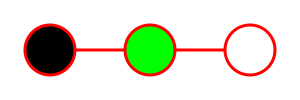
\includegraphics[width=0.12\textwidth]{img/graph/g01r.png}}	& $g_1$ & $h_1$ \\
				\raisebox{-.3\height}{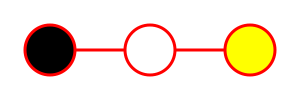
\includegraphics[width=0.12\textwidth]{img/graph/g03r.png}}	& $g_2$ & $h_2$ \\
				\raisebox{-.5\height}{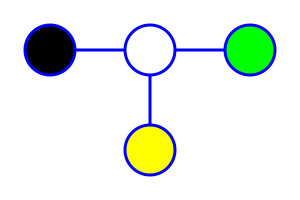
\includegraphics[width=0.12\textwidth]{img/graph/g05b.png}}	& $g_3$ & $h_3$ \\
				\raisebox{-.5\height}{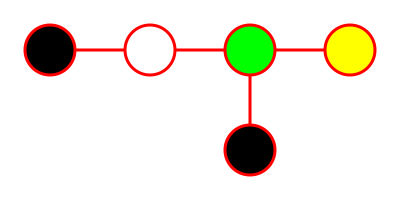
\includegraphics[width=0.12\textwidth]{img/graph/g07r.png}}	& $g_4$ & $h_4$ \\
			\end{tabular}
	\end{textblock*}



\end{tcolorbox}
